%
\section{RDBMS}
\label{sec:rdbms}
A database is a collection of data, typically describing the activities of one
or more related organizations. For example, a university database might contain
information about the following~\cite{ramakrishnan2003database}:
\begin{item-c}
\item \emph{Entities}: such as students, faculty, courses and classrooms
\item \emph{Relationships} between entities: such as students' enrollment in
  courses, faculty teaching courses, and the use of rooms for courses.
\end{item-c}

An \acrfull{dbms} is a software designed to assist in maintaining and utilizing
large collections of data.
A \acrfull{rdbms} is a subset of \gls{dbms} with relationship between tables (entities)
and rows (entities' attributes). It follows the relational model, introduced by E.F. Codd in 1970~\cite{ramakrishnan2003database},
instead of navigational model, where in the data is stored in multiple tables.
The tables are related to each other
using primary and foreign keys. It is the most used database model widely used
by enterprises and developers for storing complex and huge amounts of
data~\cite{ramakrishnan2003database}. Some examples of \gls{rdbms} are Oracle Database,
MySQL, IBM DB2, SQLite, PostgreSQL, and MariaDB.

From the users' application standpoint, a \gls{rdbms} is a management system
for databases, but is useless unless it provides an efficient and easy method to
pose questions involving the data stored in the databases. These questions are
called queries~\cite{ramakrishnan2003database}.
A \gls{dbms} provides a
specialized language --- query language --- in which queries can be performed.
The \gls{sql} for relational databases, is now the standard.
Arguably, the most widely used form
of concurrent programming is the concurrent execution of database programs
(called transactions). Users write programs as if they are to be run by
themselves, and the responsibility for running them concurrently is given to the
\gls{dbms}~\cite{ramakrishnan2003database}.

In this section an overview is presented about \gls{rdbms} foundations:
description and storage of data in a \gls{dbms}, relational model, levels of abstraction in a \gls{dbms}, transaction management,
and the structure of a \gls{dbms}. Additionally, a brief overview over \gls{sql}
and a C++ interface is presented.

\subsection{Description and storage of data in a DBMS}
\label{sec:descr-stor-data}
The user of a \gls{dbms} is ultimately concerned about the description of
various aspects of some real-world enterprise in the form of data. There are two
important data models used~\cite{ramakrishnan2003database}:
\begin{item-c}
\item \emph{Data model}: collection of high-level data description constructs
  that hide many low-level storage details. A \gls{dbms} allows a user to define
  the data to be stored in terms of a data model, such as the \textbf{relational
  data model}. It is closer to how the \gls{dbms} stores the data.
\item \emph{Semantic data model}: more abstract, high-level data model, closer
  to human thinking, serving as an useful starting point for the database
  design. The semantic data model is subsequently translated into a database
  design in terms of the data model the \gls{dbms} actually supports.
  An example is the \emph{\acrfull{er}} model which allows the user to
  pictorially denote entities and the relationship among them. The semantic data
\end{item-c}

\subsection{Relational model}
\label{sec:relational-model}
The central data description construct in the relational model is a \emph{relation},
which can be thought as a set of
\emph{records}~\cite{ramakrishnan2003database}.
A \emph{schema} is a description of data in terms of the data model. In the
relation model, the schema for a relation specifies its name, the name of each
\emph{field} (or \emph{attribute} or \emph{column}), and the type of each
field. As an example, student information in a university database may be stored
in a relation with the following schema~\cite{ramakrishnan2003database}:
\begin{quote}
\texttt{Students(\emph{sid}: string, \emph{name}: string, \emph{login}: string, \emph{age}: integer, \emph{gpa}: real)}
\end{quote}
%
The preceding schema states that each record in the Students relation has five
fields, with field names and types as indicated. As example instance of the
student relation appears in Table~\ref{tab:relational-model-example}~\cite{ramakrishnan2003database}.
%
\begingroup
\renewcommand{\arraystretch}{0.9} % Default value: 1
\begin{table}[hbt!]
\centering
\caption{An instance of the students relation --- withdrawn from \cite{ramakrishnan2003database}}
\label{tab:relational-model-example}
\begin{tabular}{@{}lllll@{}}
\toprule
\textbf{sid} & \textbf{name} & \textbf{login} & \textbf{age} & \textbf{gpa} \\ \midrule
53666        & Jones         & jones@cs       & 18           & 3.4          \\
53688        & Smith         & smith@ee       & 18           & 3.2          \\
53650        & Smith         & smith@math     & 19           & 3.8          \\
53831        & Madayan       & madayan@music  & 11           & 1.8          \\
53932        & Guldu         & guldu@music    & 12           & 2.0          \\ \bottomrule
\end{tabular}
\end{table}
\endgroup

Each row in the Students relation is a record that describes a student,
following the schema of the Students relation. Thus, the schema can be thought
as a template for describing a student. This description can be made more
precise by specifying integrity constraints, i.e., the conditions that the
records in a relation must satisfy~\cite{ramakrishnan2003database}.
For example, one could specify that every
student had a unique \texttt{sid} value, thus making a potential candidate for a
primary key, i.e., an unique identifier that univocally identifies each record
in a relation. This information cannot be captured by simply adding another
field to the Students schema, thus requiring integrity constraints to increase
the expressiveness of the constructs of a data model~\cite{ramakrishnan2003database}.

\subsection{Levels of abstraction in a DBMS}
\label{sec:levels-abstr-dbms}
The data in a \gls{dbms} is described at three levels of abstraction, as
illustrated in Fig.~\ref{fig:dbms-abstraction-levels},
namely~\cite{ramakrishnan2003database}:
\begin{item-c}
\item \emph{External schema}: allow data access to be customized (and
  authorized) at the level of individual users or group of users.
  Any given database has exactly one conceptual schema and one
physical schema because it has just one set of stored relations, but it may have
several external schemas, each tailored to a particular group of users.
Each external schema consists of a collection of one or more views and relations
from the conceptual schema.
A \emph{view} is conceptually a relation, but the records in a view are not
stored in the DBMS. Rather, they are computed using a definition for the view,
in terms of relations stored in the DBMS.
\item \emph{Conceptual schema}: also known as the \emph{logical schema},
  describes the stored data in terms of the data model of the \gls{dbms}. In a
  \gls{rdbms}, the conceptual schema describes all relations that are stored in
  the database. The conceptual schema may be design using the \gls{er} model.
\item \emph{Physical schema}: translates how the relations described in the
  conceptual schema are actually stored on secondary storage devices such as
  disks and tapes. Decisions about the physical schema are based on the
  understanding of how the data is typically accessed, typically requiring the
  design to decide about the file organizations used to store the relations and
  to create auxiliary data structures called \emph{indexes} to speed up data
  retrieval operations.
\end{item-c}
%
\begin{figure}[htb!]
\centering
    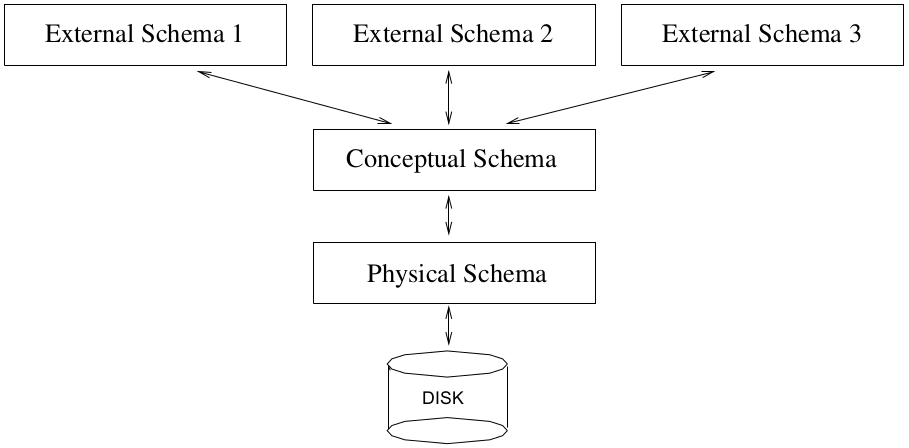
\includegraphics[width=0.65\columnwidth]{./img/dbms-abstraction-levels.png}
  \caption{Levels of abstraction in a DBMS (withdrawn from~\cite{ramakrishnan2003database})}%
\label{fig:dbms-abstraction-levels}
\end{figure}
%
\subsection{Transaction management}
\label{sec:trans-manag}
An important task of a \gls{dbms} is to schedule concurrent accesses to data in
a safe and seamless way to the user. Such accesses are named
\emph{transactions}, i.e., any one execution of a user program in a \gls{dbms},
corresponding to the basic unit of change as seen by the \gls{dbms}. Partial
transactions are not allowed, and the effect of a group of transactions is
equivalent to some serial execution of all transactions~\cite{ramakrishnan2003database}.

For the concurrent execution of transactions to take place, a \emph{locking
  protocol} is enforced by the \gls{dbms}, establishing a set of rules to be
followed by each transaction, using a \emph{lock} --- a mechanism to control
access to database objects.
Two kinds of locks are commonly supported by a DBMS: \emph{shared locks} on an
object can be held by two different transactions at the same time, but an
\emph{exclusive lock} on an object ensures that no other transactions hold any
lock on this object~\cite{ramakrishnan2003database}.

Transactions can be interrupted before running to completion for a variety of
reasons, e.g., a system crash. A DBMS must ensure that the changes made by such
incomplete transactions are removed from the database. To do so, the DBMS
maintains a log of all writes to the database, even before
the corresponding change is reflected in the database itself, enabling the
\gls{dbms} to detect and undo the changes if a system crash occurs. This property is called \gls{wal}. To ensure this property, the
DBMS must be able to selectively force a page in memory to disk~\cite{ramakrishnan2003database}.

The log is also used to ensure that the changes made by a successfully completed
transaction are not lost due to a system crash, as explained. Bringing
the database to a consistent state after a system crash can be a slow process,
since the DBMS must ensure that the effects of all transactions that completed
prior to the crash are restored, and that the effects of incomplete transactions
are undone. The time required to recover from a crash can be reduced by
periodically forcing some information to disk; this periodic operation is called a \emph{checkpoint}~\cite{ramakrishnan2003database}.

Summarizing, the main takeaways for \gls{dbms} support for concurrency control
and recovery are~\cite{ramakrishnan2003database}:
\begin{item-c}
\item \emph{Locking}:
every object that is read or written by a transaction is first locked in shared
or exclusive mode, respectively. Placing a lock on an object restricts its
availability to other transactions and thereby affects performance.
\item \emph{\gls{wal}}: for efficient log maintenance, the DBMS must be able to
  selectively force a collection of pages in main memory to disk. \gls{os}
  support for this operation is not always satisfactory.
\item \emph{Periodic checkpoint}:
  can reduce the time needed to recover from a crash. There is a trade-off
  between speed and system integrity, as checkpointing too often slows
  down normal execution. 
\end{item-c}
%
\subsection{Structure of a RDBMS}
\label{sec:structure-rdbms}

Fig.~\ref{fig:dbms-abstraction-levels} shows the structure (with some
simplification) of a typical \gls{dbms} based on the relational data model.
%
\begin{figure}[htb!]
\centering
    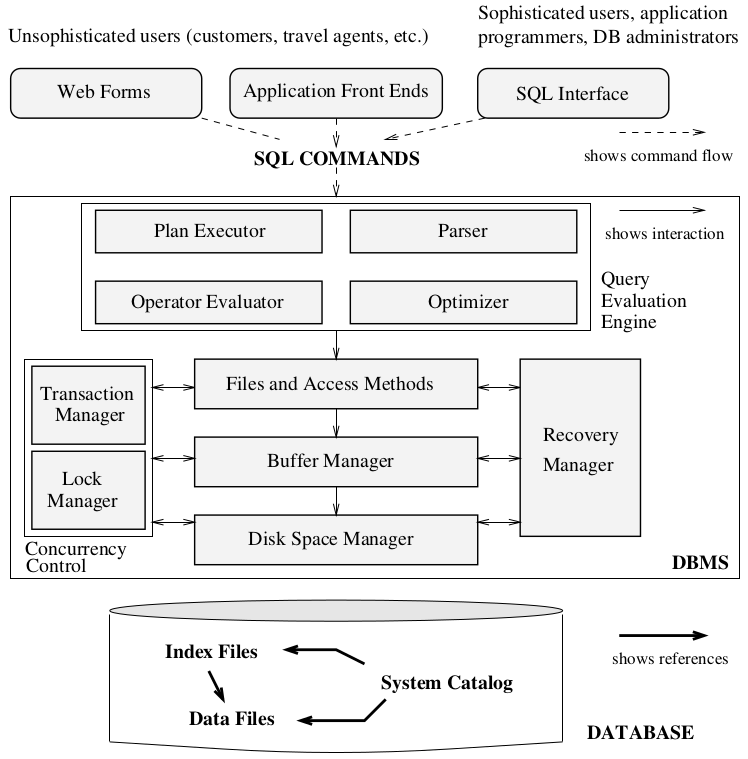
\includegraphics[width=0.75\columnwidth]{./img/dbms-struct.png}
  \caption{Architecure of a DBMS (withdrawn from~\cite{ramakrishnan2003database})}%
\label{fig:dbms-abstraction-levels}
\end{figure}
%

It is comprised of~\cite{ramakrishnan2003database}: 
\begin{item-c}
\item \emph{Interfaces}:
  The DBMS accepts \gls{sql} commands generated from a
  variety of user interfaces, produces query evaluation plans, executes these
  plans against the database, and returns the answers. SQL commands can also be
  embedded in host-language application programs, e.g., Java or C++ programs,
  but here one concentrates only on the core DBMS functionality.
\item \emph{\gls{dbms}}: contains:
  \begin{itemize}
  \item \emph{Query Evaluation Engine}:
    When a user issues a query, the parsed query is presented to a query
    optimizer, which uses information about how the data is stored to produce an
    efficient execution plan for evaluating the query. An execution plan is a
    blueprint for evaluating a query, and is usually represented as a tree of
    relational operators (with annotations that contain additional detailed
    information about which access methods to use, etc.).
  \item \emph{Concurrency control}:
  The \emph{Transaction Manager} ensures that transactions request and release
  locks according to a suitable locking protocol and schedules the execution
  transactions.
%
  The \emph{Lock Manager} keeps tracks of request for locks and grants locks on
  database objects when they become available.
 % 
  \item \emph{Recovery manager}:
    responsible for maintaining a log, and restoring the system to a consistent
    state after a crash.
  \item \emph{Disk access manager}:
    The \emph{file and access methods} layer includes a variety of software for
    supporting the concept of a file, which, in a DBMS, is a collection of pages
    or a collection of records. This layer typically supports a heap file, or
    file of unordered pages, as well as indexes.
    In addition to keeping track of the pages in a file, this layer organizes
    the information within a page.
%
    The \emph{Buffer manager} handles pages as a response to read requests.
%   
    The \emph{disk space manager} deals with management of space on
    disk, where the data is stored. Higher layers allocate, deallocate, read,
    and write pages through (routines provided by) this layer.
  \end{itemize}
\item \emph{Database}: contains the system catalog information consisting of the
  index files referencing the data files storing the actual data on physical
  memory.
\end{item-c}

\subsection{Database design overview}
\label{sec:datab-design-overv}
%
The database design process can be divided into six steps, namely~\cite{ramakrishnan2003database}:
\begin{enum-c}
\item \emph{Requirements Analysis}:
  the requirements for the database
  application are elicited and analyzed assessing what data is to be stored in
  the database, what applications must be built on top of it, and what operations are most frequent and subject to performance
  requirements.
Several methodologies have been proposed for organizing and presenting the
information gathered in this step, and some automated tools have been developed
to support this process.
\item \emph{Conceptual Database Design}:
the information gathered in the previous step is used to develop a high-level
description of the data to be stored in the database, along with the constraints that are known to hold over this data. This
step is often carried out using the \gls{er} model, or a similar high-level data model.
\item \emph{Logical Database Design}:
  A DBMS must be chosen to implement the database
design, and convert the conceptual database design -- \gls{er} schema --- into a database schema in the
data model of the chosen DBMS --- relational schema.
\item \emph{Schema Refinement}:
  Next, the collection of relations in the relation database schema are analyzed
  to identify potential problems, and to refine it. This is performed by
  normalizing relations, restructuring them to ensure some desirable
  properties.
\item \emph{Physical Database Design}:
  In this step, the typical expected workloads that the database must support
  are analyzed and further refine the database design to ensure that it meets
  desired performance criteria. This may simply involve building indexes on some tables and clustering some tables, or it may involve a substantial
  redesign of parts of the database schema obtained from the earlier design steps.
\item \emph{Security Design}:
  Lastly, the different user groups and different
roles played by various users are identified (e.g., the development team for a
product, the customer support representatives, the product manager).
For each role and user group, the permitted and forbidden parts of the database
are identified and the policies are enforced to ensure this. A DBMS provides
several mechanisms to assist in this step.
\end{enum-c}
%
\subsection{Entity-Relationship model}
\label{sec:entity-relat-model}
%
The \acrfull{er} data model enables the description of the data involved in a
real-world enterprise in terms of entities and their relationships and is widely
used to develop an initial database design. The \gls{er} model is most relevant
to the first three steps of the database
design~\cite{ramakrishnan2003database}~(see Section~\ref{sec:datab-design-overv}).
In this section are presented the
key concepts for the \gls{er} model as a database design modeling tool.
%

\subsubsection{Key concepts}
\label{sec:key-concepts}
It is important to understand some key concepts for the \gls{er} model, namely~\cite{ramakrishnan2003database}:
\begin{item-c}
\item \emph{Entity}: is an object in the real world that is distinguishable from
  other objects, e.g., the Pokemon toy, the toy department, the manager of the
  toy department, etc.
\item \emph{Entity set}: collection of entities. They do not need to be
  disjoint, i.e., entities can simultaneously belong to different entity
  sets. For example, one can define an entity set called \texttt{Employees} that
  contain both the toy and appliance department employee sets.
  An entity set is represented by a rectangle in the \gls{er} model.
\item \emph{Attributes}: an entity is described using a set of attributes. All
  entities in a given entity set have the same attributes. For example, the
  \texttt{Employees} entity set could use \texttt{name}, social security number
  (\texttt{ssn}) and parking lot (\texttt{lot}) as attributes.
  An attribute is represented by an oval in the \gls{er} model.
\item \emph{Domain}: for each attribute associated with a set, one must identify
  a domain of possible values. For example, the domain associated with the
  attribute \texttt{name} of \texttt{Employees} might be the set of 20-character
  strings.
  The domain information can be listed along the attribute name.
\item \emph{Key}: minimal set of attributes whose values uniquely identify an
  entity in the set. There could be more than one \emph{candidate} key: if so,
  one designate one of them as the \emph{primary} key.
  Each attribute in the primary key is underlined in the \gls{er} model. The
  \emph{foreign key} is(are) the
  attribute(s) which in a relationship one-to-many is(are) primary key(s) in the
  entity of the side \texttt{one} and integrates the set of attributes of the
  entity in the side \texttt{many} of that relationship
\item \emph{Relationship}: association between two or more entities.
  For example, one may have the relationship that Joe works in the pharmacy
  department.
  A relationship is represented by a straight line in the \gls{er} model and may
  also have \emph{descriptive attributes}.
\item \emph{Relationship set}: collection of similar relationships.
\item \emph{Key constraints}: restrictions over entities.
  For example, the restriction that each department has at most one manager, and
  is denoted by using an arrow from the entity to the relationship.
\item \emph{Participation constraints}: states the participation of an entity
  set in the relationship. It can be \emph{partial} or \emph{total}.
  For example, if every department is required to have a manager, the
  participation of the entity set \texttt{Departments} in the relationship set
  \texttt{Manages} is said to be \emph{total}.
\item \emph{Class hierarchies}: classification of entities in an entity set into
  subclasses, using the relationship \emph{is a}. For example, a \texttt{Car}
  \texttt{is a} \texttt{Vehicle} and a \texttt{Truck} \texttt{is a}
  \texttt{Vehicle} too. 
\item \emph{Aggregation}: indicates that a relationship set (identified through
  a dashed box) participates in another relationship set.
\end{item-c}

The \glspl{erd} use a graphical conventional to quickly and clearly depict the
entities involved and how they relate to each other. In a \gls{erd} entities are
represented by rectangles, attributes by ellipses, and the relationships as
lines between entities. In the rectangles and ellipses are placed the names of
the different entities and attributes. The relationships have cardinalities --- \texttt{1:1}
(one-to-one), \texttt{1:M} (one-to-many), and \texttt{M:N} (many-to-many) ---
and may be mandatory or optional --- e.g., a vehicle may not have any parking
space assigned, but to each parking space is assigned one, and one only,
vehicle.

Several notations can be used, namely, crow's foot, \gls{uml}, Chen, Barker,
etc~\cite{crowsfootNotation}.
In crow's foot notation:
\begin{item-c}
\item A multiplicity of one and a mandatory relationship is represented by a
  straight line perpendicular to the relationship line.
\item A multiplicity of many is represented by the three-pronged `crow-foot'
  symbol.
\item An optional relationship is represented by an empty circle.
\end{item-c}

Fig.~\ref{fig:erd-example} illustrates an example of an \acrfull{erd} using
crow's foot notation for an a company. There are three entity sets ---
\texttt{Customers}, \texttt{Orders}, and \texttt{Shipments}. Within each of
these are the attributes, with the primary key being underlined. Additionally it
also indicates the foreign key that resolves the \texttt{one-to-many}
relationship. Thus, a customer can place \texttt{0} or \texttt{many} orders, which, in
turn, can have \texttt{0} or \texttt{many} shipment methods.

%
\begin{figure}[htb!]
\centering
    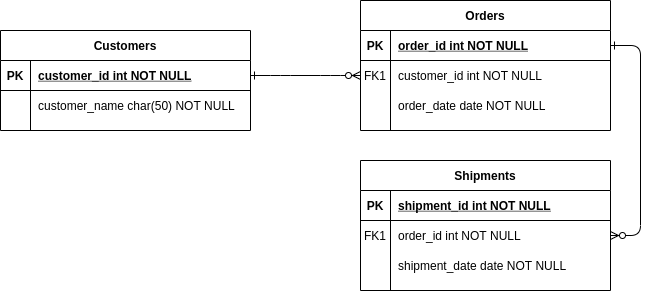
\includegraphics[width=0.8\columnwidth]{./img/erd-example.png}
  \caption{Example of an \gls{erd}}%
\label{fig:erd-example}
\end{figure}
%




\subsection{Choice of the RDBMS}
\label{sec:choice-rdbms}
In this section are presented the most relevant \glspl{rdbms}, its advantages
and disadvantages, and the best use case, which can help the database designer
to appropriately choose a \gls{rdbms}. Special focus is given to the free
systems, namely \texttt{MySQL} and\texttt{SQLite}, due to budget restrictions.

The most relevant \glspl{rdbms} are~\cite{modernDBChoice}:
% src: https://www.xplenty.com/blog/which-database/
\begin{item-c}
\item \textbf{Oracle Database}: 
Oracle has provided high-quality database solutions since the 1970s. The most
recent version of Oracle Database was designed to integrate with cloud-based
systems, and it allows you to manage massive databases with billions of
records.
    \begin{itemize}
    \item \emph{Advantages}: the most advanced technology and a wide range of
    solutions.
    \item \emph{Disadvantages}: an expensive solution and system upgrades might be
    required ---  many businesses have to upgrade their hardware before using Oracle
    solutions.
    \item \emph{Best use case}: if you're a large organization that needs to manage
    a massive amount of data, Oracle could be the ideal choice.
  \end{itemize}
\item \textbf{Microsoft SQL Server}: it is a database engine that is compatible
  with, both, on-site and cloud-based servers, and supports Windows and Linux
  OSes.
    \begin{itemize}
    \item \emph{Advantages}: it is mobile: this database engine allows you to
      access dashboard graphics and visuals via mobile devices. It integrates
      with Microsoft products.  It is fast and stable.
    \item \emph{Disadvantages}: an expensive solution and requires a lot of
      \gls{hw} resources.
    \item \emph{Best use case}: if you're an enterprise-level corporation that
      relies heavily on Microsoft products, the speed, agility, and reliability
      of Microsoft SQL Server could be an excellent choice.
  \end{itemize}
\item \textbf{MySQL}: MySQL is a free, open-source RDBMS solution that Oracle
  owns and manages. Even though it's freeware, MySQL benefits from frequent
  security and features updates. Large enterprises can upgrade to paid versions of MySQL to benefit from additional features and user support.
    \begin{itemize}
    \item \emph{Advantages}: it is open-source, free of charge (freeware) and
      highly compatible with many other database systems.
    \item \emph{Disadvantages}: lacking features common to other \glspl{rdbms}:
      because MySQL prioritizes speed and agility over features, some of the
      standard features found in other solutions may be missing, e.g., the
      ability to create incremental backups. Challenges getting quality support:
      The free version of MySQL does not come with on-demand support. However,
      MySQL does have an active volunteer community, useful forums, and a lot of
      documentation.
    \item \emph{Best use case}: MySQL is a particularly valuable RDBMS solution
      for businesses that need a solution with enterprise-level capabilities,
      but are operating under strict budget constraints. It is an extremely
      powerful and reliable modern RDBMS with a free tier.
  \end{itemize}
\item \textbf{SQLite}~\cite{MysqlVsSqlite}: it is a C-language library that
  implements a small, fast, self-contained SQL database engine --- 
  an embedded \gls{db} --- which means the \gls{db} engine runs as a part of the
  app.
    \begin{itemize}
    \item \emph{Advantages}: it is open-source, free of charge (freeware), a
      server-less and file-based database, and self-contained. It has a small
      storage footprint (the \texttt{SQLite} library is 250 KB in size, while the \texttt{MySQL}
      server is about 600 MB). It directly stores information into a single
      file, making it easy to copy, and no configuring is required.
    \item \emph{Disadvantages}: it lacks user management (not suitable for
      multiple users) and security features (the database can be accessed by
      anyone). It is not easily scalable and cannot be customized.
    \item \emph{Best use case}: \texttt{SQLite} is best suited for developing
      small standalone apps or smaller projects which do not require much
      scalability.
  \end{itemize}
\end{item-c}
%
\paragraph{\textbf{Summary}}
\texttt{Oracle Database} and \texttt{Microsoft SQL server} are proprietary
solutions, specially suited for large organizations, and can be very
expensive. On the other hand, \texttt{MySQL} and \texttt{SQLite} are open-source
and freeware solutions, which can be used to quickly test and iterate the
\gls{db} design before moving into production. However, \texttt{SQLite} does not
have user authentication or security features, and it is not easily
scalable. Thus, \texttt{MySQL} arises as the best option, suited for distributed
architectures, as a trade-off between cost, ease of use, scalability, security
and user management.
%
\subsection{SQL}
\label{sec:sql}
Ideally, a database language allows the creation of a database and table
structures, the execution of basic data management tasks (add, delete, and
modify), and the execution of complex queries designed to transform the raw data
into useful information. Moreover, it must provide a clear and easy suntax, it
must be portable and conform to some basic standard. \gls{sql} complies well to
these requirements~\cite{coronel2016database}.

\gls{sql} functions fit into two broad categories~\cite{coronel2016database}:
\begin{enum-c}
\item It is a \emph{\gls{ddl}}: SQL includes commands to create database objects
  such as tables, indexes, and views, as well as commands to define access
  rights to those database objects (see Fig.~\ref{fig:sql-dll}).
\item It is a \emph{\gls{dml}}: SQL includes commands to insert, update, delete,
  and retrieve data within the database tables (see Fig.~\ref{fig:sql-dml}).
\end{enum-c}
%
\begin{figure}[htb!]
\centering
    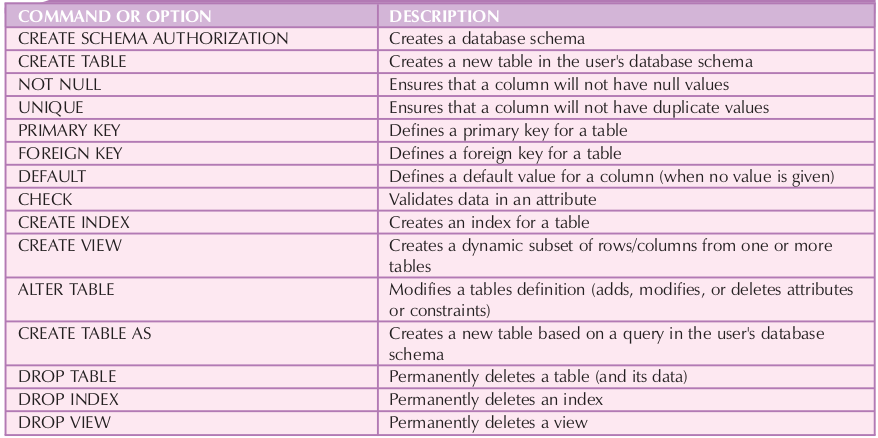
\includegraphics[width=0.9\columnwidth]{./img/sql-dll.png}
  \caption{SQL data definition commands --- withdrawn from~\cite{coronel2016database}}%
  \label{fig:sql-dll}
\end{figure}
%
\begin{figure}[htb!]
  \centering
  % 
  \begin{subfigure}[t]{.9\textwidth}
  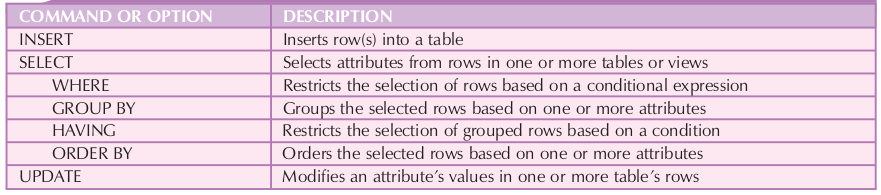
\includegraphics[width=\textwidth]{img/sql-dml-1.png}%
  %\caption{main}%
  %\label{fig:state-mach-local-superv-main}
\end{subfigure}
%
%\vspace{-0.1\textwidth}
%
  \begin{subfigure}{.9\textwidth}
  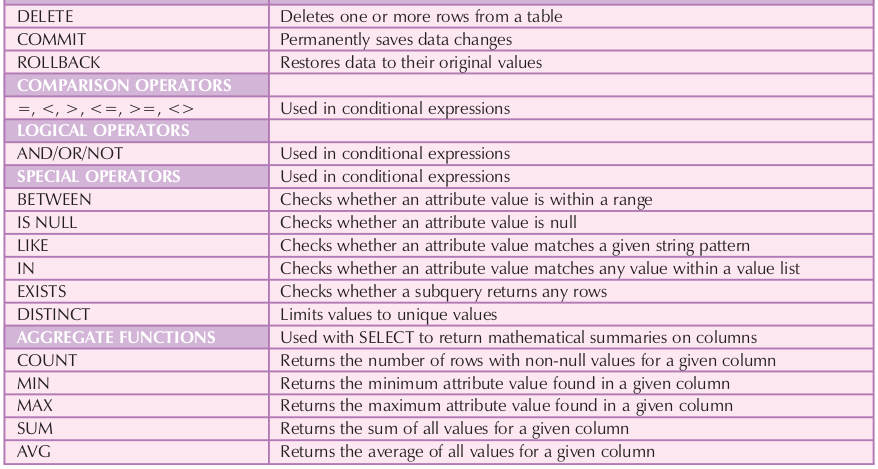
\includegraphics[width=\textwidth]{img/sql-dml-2.png}%
  %\caption{Mode Manager}%
  %\label{fig:state-mach-local-superv-mode}
\end{subfigure}
  % 
  \caption{SQL data manipulation commands --- withdrawn from~\cite{coronel2016database}}%
  \label{fig:sql-dml}
\end{figure}
%


\subsection{MySQL Interfaces}
\label{sec:sql-interfaces}
\texttt{MySQL} works under the client--server paradigm. It has several client
interfaces that can interact with the server, through connectors and
\glspl{api}, i.e., the drivers and libraries that one can use to connect
applications in different programming languages to \texttt{MySQL} database
servers.
The application and database server can be on the same machine, or communicate
across the network~\cite{MysqlConnAPIs}.
The following interfaces are available: \texttt{Java}, \texttt{Python},
\texttt{JavaScript}, \texttt{C++}, \texttt{C},
\texttt{C\#},
\texttt{PHP},
\texttt{OBDC}, \texttt{NBD Cluster},
\texttt{MySQL Shell}, and \texttt{X DevAPI}.

\subsubsection{C++ connector}
\label{sec:c++-connector}
From the list of available interfaces, the most well suited to interface the
\gls{rdbms} are the \texttt{C \gls{api}} and the \texttt{C++ connector}, as they
are the most well known programming languages by the authors and the better ones
in terms of performance.
However, the \texttt{C++ connector} was chosen because it offers the following
benefits over the MySQL C API provided by the MySQL client library~\cite{MysqlConnC++Intro}:
\begin{item-c}
\item Convenience of pure C++.
\item Support for the object-oriented programming paradigm.
\item Support for these application programming interfaces: X DevAPI, X DevAPI
  for C, Legacy JDBC 4.0-based API.
\item Reduced development time.
\item Licensed under the GPL with the FLOSS License Exception.
\item Available under a commercial license upon request.
\end{item-c}



%% Local Variables:
%% mode: latex
%% TeX-master: "../../../dissertation"
%% End:
